\section{Results and Discussion}
\begin{figure}[!htbp]
\begin{center}
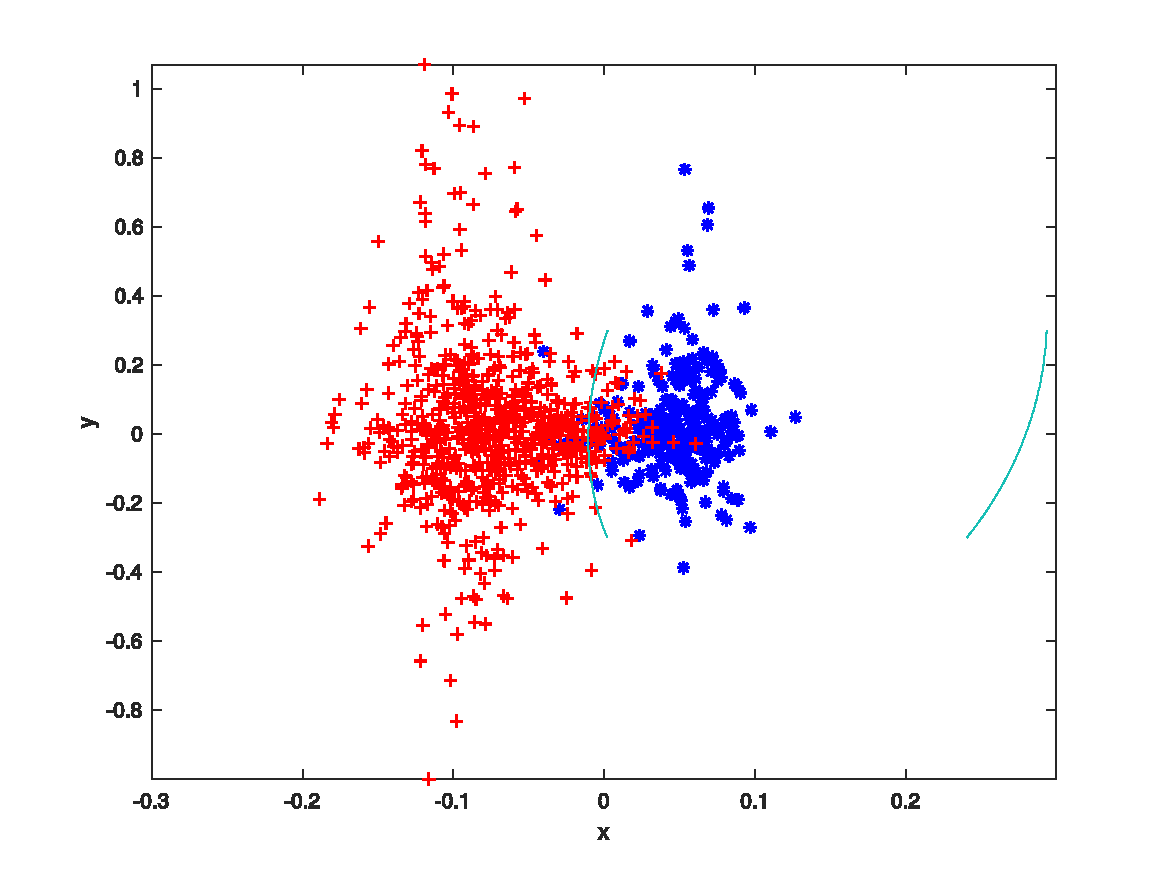
\includegraphics[width=\textwidth]{img/clean_boundary.pdf}
\caption{
Plot of LDA-transformed bag-of-words data from the ``dirty'' dataset.
``Helpful'' reviews are shown in blue and ``not helpful'' reviews are shown in red.
The Bayes decision boundary generated when these data are modeled as drawn from multivariate Gaussian distributions is depicted in turquoise.
}
\label{fig:clean_boundary}
\end{center}
\end{figure}

\begin{figure}[!htbp]
\begin{center}
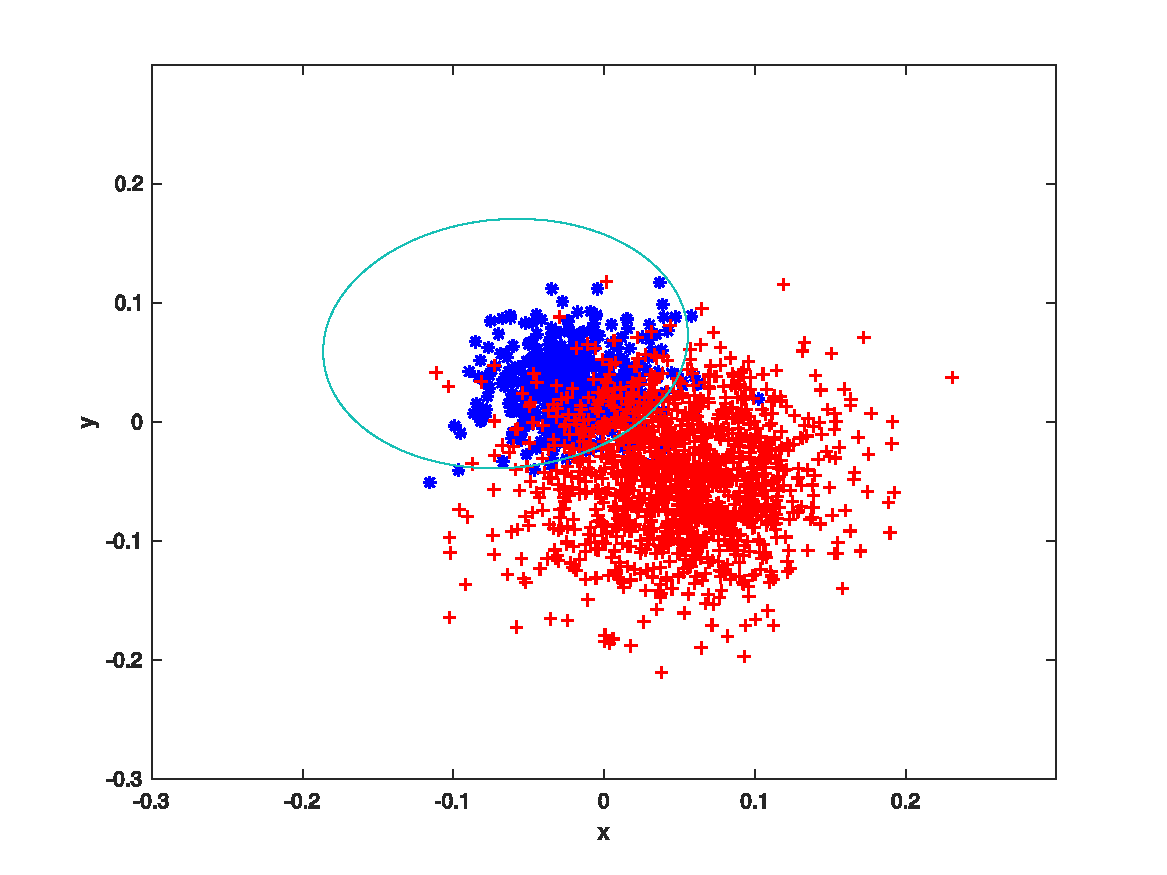
\includegraphics[width=\textwidth]{img/dirty_boundary.pdf}
\caption{
Plot of LDA-transformed bag-of-words data from the ``dirty'' dataset.
``Helpful'' reviews are shown in red and ``not helpful'' reviews are shown in blue.
The Bayes decision boundary generated when these data are modeled as drawn from multivariate Gaussian distributions is depicted in turquoise.
}
\label{fig:dirty_boundary}
\end{center}
\end{figure}

\begin{figure}[!htbp]
\begin{subfigure}[b]{0.5\textwidth}
\begin{center}
\newcommand\items{2}   %Number of classes
\noindent\begin{tabular}{cc*{\items}{|E}|J}
\multicolumn{1}{c}{} &\multicolumn{1}{c}{} &\multicolumn{\items}{c}{Predicted} \\
\multicolumn{1}{c}{} &
\multicolumn{1}{c|}{} &
\multicolumn{1}{c|}{} &
\multicolumn{1}{c|}{NOT} \\
\multicolumn{1}{c}{} &
\multicolumn{1}{c|}{} &
\multicolumn{1}{c|}{HELPFUL} &
\multicolumn{1}{c|}{HELPFUL} \\

\hhline{~-*{\items}{|-}|}
\multirow{\items}{*}{\rotatebox{90}{Actual}}
& HELPFUL & 126 & 37 & \\[0.6cm]
\hhline{~-*{\items}{|-}|}
& NOT HELPFUL & 21 & 18 & \\[0.6cm]
\hhline{~-*{\items}{|-}|}
\end{tabular}
\caption{``dirty'' dataset}
\end{center}
\end{subfigure}%
\begin{subfigure}[b]{0.5\textwidth}
\begin{center}
\newcommand\items{2}   %Number of classes
\noindent\begin{tabular}{cc*{\items}{|E}|J}
\multicolumn{1}{c}{} &\multicolumn{1}{c}{} &\multicolumn{\items}{c}{Predicted} \\
\multicolumn{1}{c}{} &
\multicolumn{1}{c|}{} &
\multicolumn{1}{c|}{} &
\multicolumn{1}{c|}{NOT} \\
\multicolumn{1}{c}{} &
\multicolumn{1}{c|}{} &
\multicolumn{1}{c|}{HELPFUL} &
\multicolumn{1}{c|}{HELPFUL} \\
\hhline{~-*{\items}{|-}|}
\multirow{\items}{*}{\rotatebox{90}{Actual}}
& HELPFUL & 487 & 239 & \\[0.6cm]
\hhline{~-*{\items}{|-}|}
& NOT HELPFUL & 164 & 107 & \\[0.6cm]
\hhline{~-*{\items}{|-}|}
\end{tabular}
\caption{``clean'' dataset}
\end{center}
\end{subfigure}
\caption{
Test data confusion matrices of Bayes classification with multivariate Gaussian models of distribution on ``dirty'' and ``clean'' datasets. 
}
\label{fig:confusion_bayes}
\end{figure}

\begin{figure}[!htbp]
\begin{subfigure}[b]{0.5\textwidth}
\begin{center}
\newcommand\items{2}   %Number of classes
\noindent\begin{tabular}{cc*{\items}{|E}|J}
\multicolumn{1}{c}{} &\multicolumn{1}{c}{} &\multicolumn{\items}{c}{Predicted} \\
\multicolumn{1}{c}{} &
\multicolumn{1}{c|}{} &
\multicolumn{1}{c|}{} &
\multicolumn{1}{c|}{NOT} \\
\multicolumn{1}{c}{} &
\multicolumn{1}{c|}{} &
\multicolumn{1}{c|}{HELPFUL} &
\multicolumn{1}{c|}{HELPFUL} \\

\hhline{~-*{\items}{|-}|}
\multirow{\items}{*}{\rotatebox{90}{Actual}}
& HELPFUL & 127 & 38 & \\[0.6cm]
\hhline{~-*{\items}{|-}|}
& NOT HELPFUL & 19 & 16 & \\[0.6cm]
\hhline{~-*{\items}{|-}|}
\end{tabular}
\caption{``dirty'' dataset}
\end{center}
\end{subfigure}%
\begin{subfigure}[b]{0.5\textwidth}
\begin{center}
\newcommand\items{2}   %Number of classes
\noindent\begin{tabular}{cc*{\items}{|E}|J}
\multicolumn{1}{c}{} &\multicolumn{1}{c}{} &\multicolumn{\items}{c}{Predicted} \\
\multicolumn{1}{c}{} &
\multicolumn{1}{c|}{} &
\multicolumn{1}{c|}{} &
\multicolumn{1}{c|}{NOT} \\
\multicolumn{1}{c}{} &
\multicolumn{1}{c|}{} &
\multicolumn{1}{c|}{HELPFUL} &
\multicolumn{1}{c|}{HELPFUL} \\
\hhline{~-*{\items}{|-}|}
\multirow{\items}{*}{\rotatebox{90}{Actual}}
& HELPFUL & 476 & 249 & \\[0.6cm]
\hhline{~-*{\items}{|-}|}
& NOT HELPFUL & 162 & 109 & \\[0.6cm]
\hhline{~-*{\items}{|-}|}
\end{tabular}
\caption{``clean'' dataset}
\end{center}
\end{subfigure}
\caption{
Test data confusion matrices of 1 nearest neighbor classification on ``dirty'' and ``clean'' datasets. 
}
\label{fig:confusion_1nn}
\end{figure}

\begin{figure}[!htbp]
\begin{subfigure}[b]{0.5\textwidth}
\begin{center}
\newcommand\items{2}   %Number of classes
\noindent\begin{tabular}{cc*{\items}{|E}|J}
\multicolumn{1}{c}{} &\multicolumn{1}{c}{} &\multicolumn{\items}{c}{Predicted} \\
\multicolumn{1}{c}{} &
\multicolumn{1}{c|}{} &
\multicolumn{1}{c|}{} &
\multicolumn{1}{c|}{NOT} \\
\multicolumn{1}{c}{} &
\multicolumn{1}{c|}{} &
\multicolumn{1}{c|}{HELPFUL} &
\multicolumn{1}{c|}{HELPFUL} \\

\hhline{~-*{\items}{|-}|}
\multirow{\items}{*}{\rotatebox{90}{Actual}}
& HELPFUL & 123 & 36 & \\[0.6cm]
\hhline{~-*{\items}{|-}|}
& NOT HELPFUL & 23 & 18 & \\[0.6cm]
\hhline{~-*{\items}{|-}|}
\end{tabular}
\caption{``dirty'' dataset}
\end{center}
\end{subfigure}%
\begin{subfigure}[b]{0.5\textwidth}
\begin{center}
\newcommand\items{2}   %Number of classes
\noindent\begin{tabular}{cc*{\items}{|E}|J}
\multicolumn{1}{c}{} &\multicolumn{1}{c}{} &\multicolumn{\items}{c}{Predicted} \\
\multicolumn{1}{c}{} &
\multicolumn{1}{c|}{} &
\multicolumn{1}{c|}{} &
\multicolumn{1}{c|}{NOT} \\
\multicolumn{1}{c}{} &
\multicolumn{1}{c|}{} &
\multicolumn{1}{c|}{HELPFUL} &
\multicolumn{1}{c|}{HELPFUL} \\
\hhline{~-*{\items}{|-}|}
\multirow{\items}{*}{\rotatebox{90}{Actual}}
& HELPFUL & 484 & 241 & \\[0.6cm]
\hhline{~-*{\items}{|-}|}
& NOT HELPFUL & 168 & 103 & \\[0.6cm]
\hhline{~-*{\items}{|-}|}
\end{tabular}
\caption{``clean'' dataset}
\end{center}
\end{subfigure}
\caption{
Test data confusion matrices of 5 nearest neighbor classification on ``dirty'' and ``clean'' datasets. 
}
\label{fig:confusion_5nn}
\end{figure}

\begin{figure}[!htbp]
\begin{subfigure}[b]{0.5\textwidth}
\begin{center}
\newcommand\items{2}   %Number of classes
\noindent\begin{tabular}{cc*{\items}{|E}|J}
\multicolumn{1}{c}{} &\multicolumn{1}{c}{} &\multicolumn{\items}{c}{Predicted} \\
\multicolumn{1}{c}{} &
\multicolumn{1}{c|}{} &
\multicolumn{1}{c|}{} &
\multicolumn{1}{c|}{NOT} \\
\multicolumn{1}{c}{} &
\multicolumn{1}{c|}{} &
\multicolumn{1}{c|}{HELPFUL} &
\multicolumn{1}{c|}{HELPFUL} \\

\hhline{~-*{\items}{|-}|}
\multirow{\items}{*}{\rotatebox{90}{Actual}}
& HELPFUL & 123 & 36 & \\[0.6cm]
\hhline{~-*{\items}{|-}|}
& NOT HELPFUL & 23 & 18 & \\[0.6cm]
\hhline{~-*{\items}{|-}|}
\end{tabular}
\caption{``dirty'' dataset}
\end{center}
\end{subfigure}%
\begin{subfigure}[b]{0.5\textwidth}
\begin{center}
\newcommand\items{2}   %Number of classes
\noindent\begin{tabular}{cc*{\items}{|E}|J}
\multicolumn{1}{c}{} &\multicolumn{1}{c}{} &\multicolumn{\items}{c}{Predicted} \\
\multicolumn{1}{c}{} &
\multicolumn{1}{c|}{} &
\multicolumn{1}{c|}{} &
\multicolumn{1}{c|}{NOT} \\
\multicolumn{1}{c}{} &
\multicolumn{1}{c|}{} &
\multicolumn{1}{c|}{HELPFUL} &
\multicolumn{1}{c|}{HELPFUL} \\
\hhline{~-*{\items}{|-}|}
\multirow{\items}{*}{\rotatebox{90}{Actual}}
& HELPFUL & 493 & 232 & \\[0.6cm]
\hhline{~-*{\items}{|-}|}
& NOT HELPFUL & 169 & 102 & \\[0.6cm]
\hhline{~-*{\items}{|-}|}
\end{tabular}
\caption{``clean'' dataset}
\end{center}
\end{subfigure}
\caption{
Test data confusion matrices of 13 nearest neighbor classification on ``dirty'' and ``clean'' datasets. 
}
\label{fig:confusion_9nn}
\end{figure}

\begin{figure}[!htbp]
\begin{subfigure}[b]{0.5\textwidth}
\begin{center}
\newcommand\items{2}   %Number of classes
\noindent\begin{tabular}{cc*{\items}{|E}|J}
\multicolumn{1}{c}{} &\multicolumn{1}{c}{} &\multicolumn{\items}{c}{Predicted} \\
\multicolumn{1}{c}{} &
\multicolumn{1}{c|}{} &
\multicolumn{1}{c|}{} &
\multicolumn{1}{c|}{NOT} \\
\multicolumn{1}{c}{} &
\multicolumn{1}{c|}{} &
\multicolumn{1}{c|}{HELPFUL} &
\multicolumn{1}{c|}{HELPFUL} \\

\hhline{~-*{\items}{|-}|}
\multirow{\items}{*}{\rotatebox{90}{Actual}}
& HELPFUL & 123 & 38 & \\[0.6cm]
\hhline{~-*{\items}{|-}|}
& NOT HELPFUL & 23 & 16 & \\[0.6cm]
\hhline{~-*{\items}{|-}|}
\end{tabular}
\caption{``dirty'' dataset}
\end{center}
\end{subfigure}%
\begin{subfigure}[b]{0.5\textwidth}
\begin{center}
\newcommand\items{2}   %Number of classes
\noindent\begin{tabular}{cc*{\items}{|E}|J}
\multicolumn{1}{c}{} &\multicolumn{1}{c}{} &\multicolumn{\items}{c}{Predicted} \\
\multicolumn{1}{c}{} &
\multicolumn{1}{c|}{} &
\multicolumn{1}{c|}{} &
\multicolumn{1}{c|}{NOT} \\
\multicolumn{1}{c}{} &
\multicolumn{1}{c|}{} &
\multicolumn{1}{c|}{HELPFUL} &
\multicolumn{1}{c|}{HELPFUL} \\
\hhline{~-*{\items}{|-}|}
\multirow{\items}{*}{\rotatebox{90}{Actual}}
& HELPFUL & 493 & 232 & \\[0.6cm]
\hhline{~-*{\items}{|-}|}
& NOT HELPFUL & 104 & 167 & \\[0.6cm]
\hhline{~-*{\items}{|-}|}
\end{tabular}
\caption{``clean'' dataset}
\end{center}
\end{subfigure}
\caption{
Test data confusion matrices of 13 nearest neighbor classification on ``dirty'' and ``clean'' datasets. 
}
\label{fig:confusion_13nn}
\end{figure}

\begin{figure}[!htbp]
\begin{subfigure}[b]{0.5\textwidth}
\begin{center}
\newcommand\items{2}   %Number of classes
\noindent\begin{tabular}{cc*{\items}{|E}|J}
\multicolumn{1}{c}{} &\multicolumn{1}{c}{} &\multicolumn{\items}{c}{Predicted} \\
\multicolumn{1}{c}{} &
\multicolumn{1}{c|}{} &
\multicolumn{1}{c|}{} &
\multicolumn{1}{c|}{NOT} \\
\multicolumn{1}{c}{} &
\multicolumn{1}{c|}{} &
\multicolumn{1}{c|}{HELPFUL} &
\multicolumn{1}{c|}{HELPFUL} \\

\hhline{~-*{\items}{|-}|}
\multirow{\items}{*}{\rotatebox{90}{Actual}}
& HELPFUL & 123 & 37 & \\[0.6cm]
\hhline{~-*{\items}{|-}|}
& NOT HELPFUL & 23 & 17 & \\[0.6cm]
\hhline{~-*{\items}{|-}|}
\end{tabular}
\caption{``dirty'' dataset}
\end{center}
\end{subfigure}%
\begin{subfigure}[b]{0.5\textwidth}
\begin{center}
\newcommand\items{2}   %Number of classes
\noindent\begin{tabular}{cc*{\items}{|E}|J}
\multicolumn{1}{c}{} &\multicolumn{1}{c}{} &\multicolumn{\items}{c}{Predicted} \\
\multicolumn{1}{c}{} &
\multicolumn{1}{c|}{} &
\multicolumn{1}{c|}{} &
\multicolumn{1}{c|}{NOT} \\
\multicolumn{1}{c}{} &
\multicolumn{1}{c|}{} &
\multicolumn{1}{c|}{HELPFUL} &
\multicolumn{1}{c|}{HELPFUL} \\
\hhline{~-*{\items}{|-}|}
\multirow{\items}{*}{\rotatebox{90}{Actual}}
& HELPFUL & 496 & 229 & \\[0.6cm]
\hhline{~-*{\items}{|-}|}
& NOT HELPFUL & 166 & 105 & \\[0.6cm]
\hhline{~-*{\items}{|-}|}
\end{tabular}
\caption{``clean'' dataset}
\end{center}
\end{subfigure}
\caption{
Test data confusion matrices of 17 nearest neighbor classification on ``dirty'' and ``clean'' datasets. 
}
\label{fig:confusion_17nn}
\end{figure}

\begin{figure}[!htbp]
\begin{subfigure}[b]{0.5\textwidth}
\begin{center}
\newcommand\items{2}   %Number of classes
\noindent\begin{tabular}{cc*{\items}{|E}|J}
\multicolumn{1}{c}{} &\multicolumn{1}{c}{} &\multicolumn{\items}{c}{Predicted} \\
\multicolumn{1}{c}{} &
\multicolumn{1}{c|}{} &
\multicolumn{1}{c|}{} &
\multicolumn{1}{c|}{NOT} \\
\multicolumn{1}{c}{} &
\multicolumn{1}{c|}{} &
\multicolumn{1}{c|}{HELPFUL} &
\multicolumn{1}{c|}{HELPFUL} \\

\hhline{~-*{\items}{|-}|}
\multirow{\items}{*}{\rotatebox{90}{Actual}}
& HELPFUL & 123 & 39 & \\[0.6cm]
\hhline{~-*{\items}{|-}|}
& NOT HELPFUL & 23 & 15 & \\[0.6cm]
\hhline{~-*{\items}{|-}|}
\end{tabular}
\caption{``dirty'' dataset}
\end{center}
\end{subfigure}%
\begin{subfigure}[b]{0.5\textwidth}
\begin{center}
\newcommand\items{2}   %Number of classes
\noindent\begin{tabular}{cc*{\items}{|E}|J}
\multicolumn{1}{c}{} &\multicolumn{1}{c}{} &\multicolumn{\items}{c}{Predicted} \\
\multicolumn{1}{c}{} &
\multicolumn{1}{c|}{} &
\multicolumn{1}{c|}{} &
\multicolumn{1}{c|}{NOT} \\
\multicolumn{1}{c}{} &
\multicolumn{1}{c|}{} &
\multicolumn{1}{c|}{HELPFUL} &
\multicolumn{1}{c|}{HELPFUL} \\
\hhline{~-*{\items}{|-}|}
\multirow{\items}{*}{\rotatebox{90}{Actual}}
& HELPFUL & 498 & 227 & \\[0.6cm]
\hhline{~-*{\items}{|-}|}
& NOT HELPFUL & 170 & 101 & \\[0.6cm]
\hhline{~-*{\items}{|-}|}
\end{tabular}
\caption{``clean'' dataset}
\end{center}
\end{subfigure}
\caption{
Test data confusion matrices of 21 nearest neighbor classification on ``dirty'' and ``clean'' datasets. 
}
\label{fig:confusion_21nn}
\end{figure}

\begin{figure}[!htbp]
\begin{center}
\begin{tabular}{ |c|c|c| } 
 \hline
 method & ``clean'' dataset & ``dirty'' dataset \\ 
 \hline
 Bayes & 40.42\% & 28.71\% \\ 
 1-nn & 41.27\% & 28.50\% \\
 5-nn & 41.06\% & 29.50\% \\ 
 9-nn & 40.26\% & 29.50\% \\ 
 13-nn & 40.06\% & 30.50\% \\ 
 17-nn & 39.66\% & 30.00\% \\ 
 21-nn & 39.86\% & 31.00\% \\
 \hline
\end{tabular}
\end{center}
\caption{
Classifier error rate on test data.
}
\label{fig:error_rates}
\end{figure}

As was mentioned before, the goal of this project was to compare parametric (Bayes) and non-parametric (KNN) classifiers on Amazon electronics reviews.
The data classified was in one of two forms: clean and dirty.
The dirty data means that words that were the same but contained different cases or punctuation were considered separate features from the root words.
For example, "The" and "the" would be considered different features in the dirty set of data.
The clean data had all words stripped of punctuation, all lowercase, and contained only the root words.
This means that "starting", "Starting", "start", and "Start" are all counted as the same root word, "start". 

For the Bayes classifier on the "dirty data" we had an error rate of 28.71\%.
In contrast, the clean data had an error rate of 40.42\% with the Bayes classifier.
The confusion matrices for the Bayes classifier approach on both datasets is provided in Figure \ref{fig:confusion_bayes}.
Notably, the ``dirty data'' Bayes classifier was generally tended to classify more test data as ``helpful'' than  the ``clean data'' Bayes classifier (72.77\% of test data classified `helpful'' vs 65.21\%).
This is closer to the true proportion of ``helpful'' reviews in the dataset, which is approximately 80\%.

All KNN classifiers performed comparably to the Bayes classifier on the ``clean'' and ``dirty'' datasets.
KNN error rates varied between 39.86\% and 41.27\% on the ``clean'' dataset and between 28.50\% and 31\% on the ``dirty'' dataset.
Interestingly, KNN performance was greatest with the highest K (21) on the ``clean'' dataset and greatest with the lowest K (1) on the ``dirty'' dataset.
In both datasets, the overall lowest error rates was achieved with KNN classification, although Bayes classification was closely competitive.
Figure \ref{fig:error_rates} summarizes the error rates for all classifiers on both datasets.
Figures \ref{fig:confusion_1nn} through \ref{fig:confusion_21nn} provide confusion matrices for all KNN classifiers on both datasets.
The same pattern as before observed in all classifiers: ``dirty data'' KNN classifiers tended to classify more test data as ``helpful'' than the ``clean data'' KNN classifiers.

As shown in Figure \ref{fig:error_rates}, we consistently observed an approximately 10\% decrease in classifier error when using the ``dirty'' dataset over the ``clean'' dataset.
Perhaps the use of certain verb conjugations, punctuation patterns, and/or capitalization schemes (i.e., didn't bother to capitalize their reviews properly) is indicative of the usefulness of a review. 
A ``helpful'' review would be one that uses proper grammar, spelling, etc. because this makes it easy to read, and therefore easier to understand and make your own judgments about. Whereas a review that looks rushed, such as being typed in all lowercase letters and not using proper punctuation,  might make it harder to understand or follow along and therefore one would not think this review is``helpful'' due to the increased time it takes to fully understand it.
It must be noted that this result might also be an artifact of the larger training sets used for the ``dirty'' data classifiers. 
While our intuitive explanation for the consistently greater performance of our classifiers on the dirty dataset is highly speculative, it is interesting that data pre-processing might actually harm the performance of natural language classifiers.
The result certainly warrants further analysis, which would be necessary to confirm our interpretation of the apparent negative effects of data-preprocessing in this context.
